% ERA-Großpraktikums: Benutzeranleitung -- Erste Schritte

\section{Erste Schritte}

\todo[inline]{Hier soll ein kurzes Tutorial hin, z.B. zur Projekterstellung,
mein erstes RISC-V Programm, etc. Vielleicht von Anfang bis Ende ein kleiner
Schnelldurchlauf, der alle Teile kurz anschneidet.  Für eine tiefergreifende
Einsicht kann dann auch das gesamte User Manual durchgelesen werden. Aber ich
denke man sollte auch einen Teil für die ''ungeduldigen'' Studenten machen ;) }

Um sich mit dem Simulator vertraut zu machen, folgt hier eine kleine Anleitung
zum Erstellen des ersten Projekts und einigen Features des Simulators.\\

Nach dem Start des Simulators kann man entweder ein bestehendes Projekt laden
oder ein neues Erstellen. Da dies das erste Projekt ist, erstellen wir ein
Projekt und nennen es ''Mein erstes RISCV Projekt''.\\

\begin{figure}[H]
	\centering
	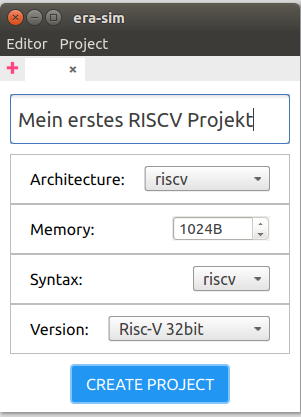
\includegraphics[scale=1.0]{Images/first-steps-1.png}
	\caption{Projekt erstellen}
\end{figure}

Nun öffnet sich das Kernstück des Simulators. Die Tabs im oberen Bereich zeigen
die zur Zeit geöffneten Projekte. Momentan ist nur unser Projekt geöffnet. Der
Texteditor ist mittig platziert. Unser simples Programm soll lediglich die
Antwort auf das Leben, das Universum und den ganzen Rest in Register x3
ausgeben. Dazu tippen wir folgende Instruktionen in den Editor:
\begin{lstlisting}
  addi x1, x0, 1
  addi x2, x0, 41
  add x3, x1, x2
\end{lstlisting}
Gültige Instruktionen werden im Editor farblich hervorgehoben. Den Farbstil kann
man durch ein neues Theme ändern (mehr dazu in
\autoref{user-manual-configuration}). In der rechts unteren Komponente werden
hilfreiche Informationen zu aktuellen Befehl angezeigt. Die selben Information
sind außerdem über das Fragezeichen-Symbol zu erreichen.

\begin{figure}[H]
	\centering
	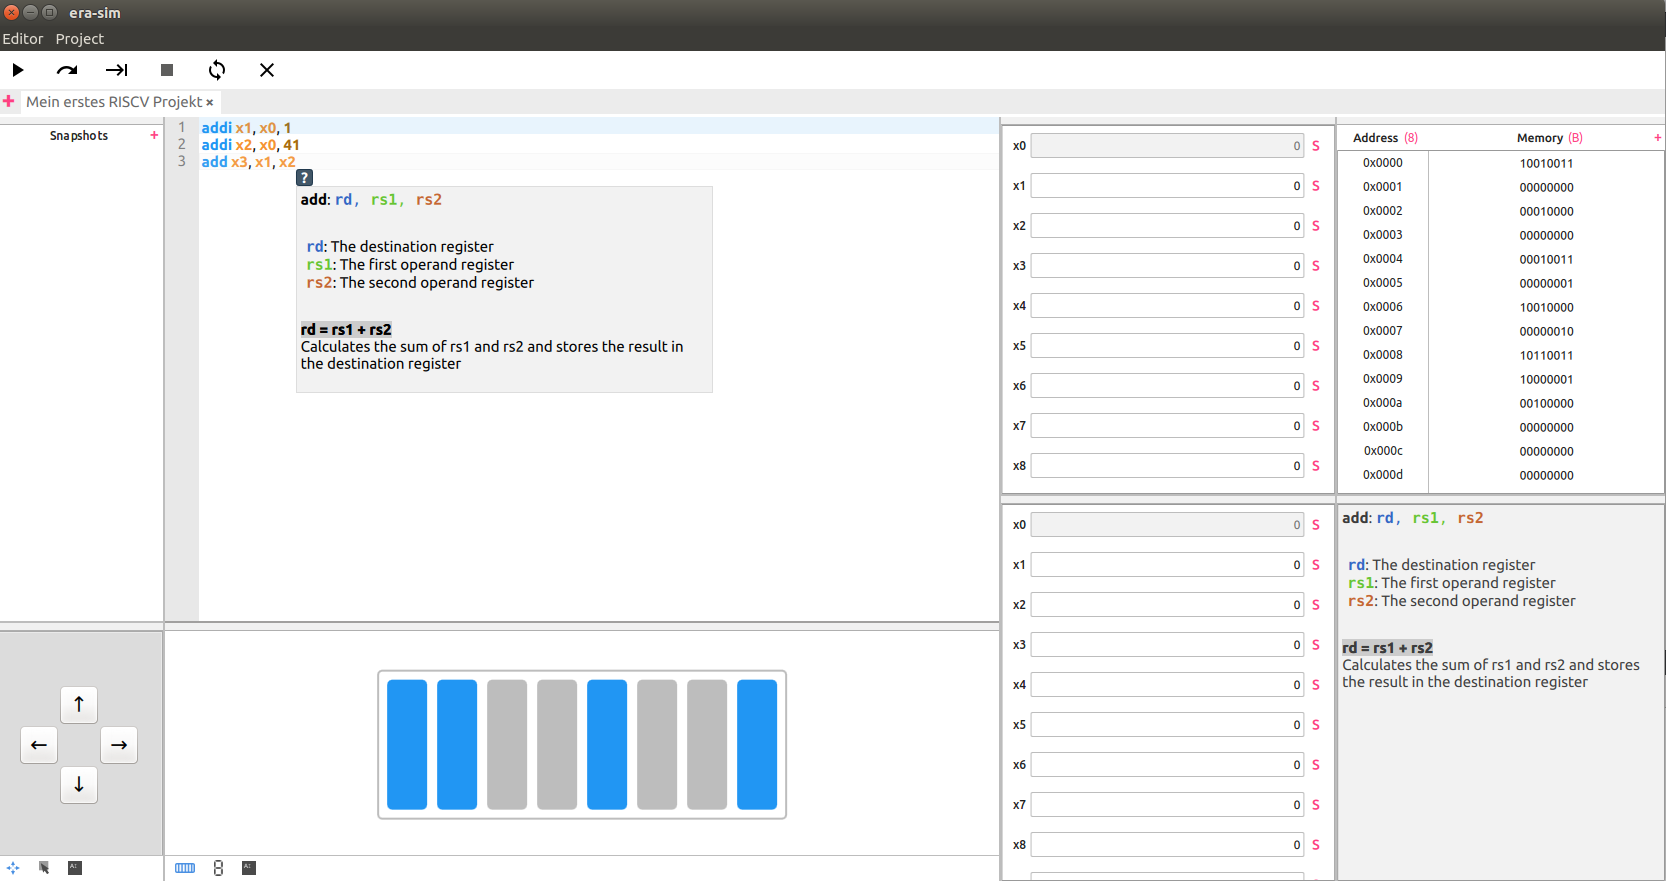
\includegraphics[scale=0.4]{Images/first-steps-2.png}
	\caption{Der Simulator}
\end{figure}

Da uns die Antwort brennend interessiert, werden wir das Programm ausführen. Das
ist möglich, da keine Übersetzungsfehler aufgetreten sind. Solche Fehler werden
als rote Nachrichten am rechten Rand des Texteditors angezeigt. In der linken
oberen Ecke befinden sich 6 Symbole, die die Ausführung steuern. Das zweite
Symbol von links -- ein gekrümmter Pfeil -- führt die nächste Instruktion aus.
Die Zeile der nächsten Instruktion ist farblich hervorgehoben. Ein Klick auf den
gekrümmten Pfeil und die Instruktion wird ausgeführt.
\begin{figure}[H]
	\centering
	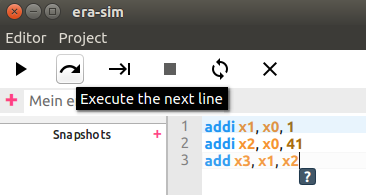
\includegraphics[scale=1.0]{Images/first-steps-3.png}
	\caption{Ausführen der nächsten Instruktion}
\end{figure}

Das Register x1 hat sich verändert. Statt 0 hat es jetzt den Wert 1. Während dem
kleinschrittigen Ausführen werden alle Änderungen an den Registern farblich
hervorgehoben.

\begin{figure}[H]
	\centering
	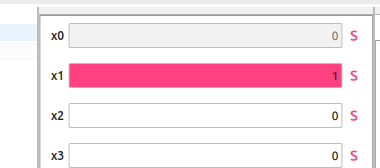
\includegraphics[scale=1.0]{Images/first-steps-4.png}
	\caption{Farbliche Hervorhebung nach erstem Schritt}
\end{figure}

Führen wir die nächsten zwei Instruktionen aus, so steht das Ergebnis in x3.
\begin{figure}[H]
	\centering
	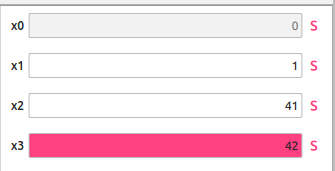
\includegraphics[scale=1.0]{Images/first-steps-5.png}
	\caption{Farbliche Hervorhebung nach drittem Schritt}
\end{figure}

Vielleicht ist es beim Tippen vorhin unbemerkt geblieben: Auch der Speicher, in
der Speicherkomponente auf der rechten Seite des Simulators hat sich verändert.
Die Speicherkomponente zeigt an, welchen Wert der Speicher an welcher Adresse
hat. Momentan wird der Wert als Binärzahl angezeigt (zu erkennen am ''B''). Mit
einem Klick auf das Plus neben der Kopfzeile der Tabelle fügen wir eine neue
Spalte ein. Ein Klick auf den Kopf der neuen Spalte bietet diverse
Anzeigemöglichkeiten. Wir wählen ''Hexadezimal'' aus. Das ''B'' an der
betreffenden Spalte hat sich nun zu einem ''H'' verwandelt.
\begin{figure}[H]
	\centering
	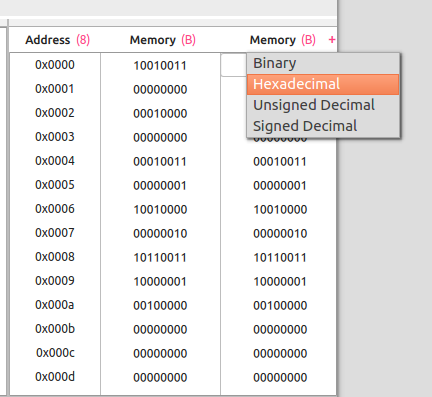
\includegraphics[scale=1.0]{Images/first-steps-6.png}
	\caption{Darstellungsarten in der Speicherkomponente}
\end{figure}

Nun erkennen wir, die Werte im Speicher sind die übersetzten (oder auch
assemblierten) Instruktionen aus dem Texteditor. Nach jeder Änderung am Code im
Texteditor wird auch der Speicher mit dem assemblierten Programm aktualisiert.\\
Jetzt werden wir das Geschriebene speichern. Dazu gibt es mehrere Einträge im
Dateimenü ''Editor''. Wir wählen einen aus und speichern den Code unter einem
Namen.
\begin{figure}[H]
	\centering
	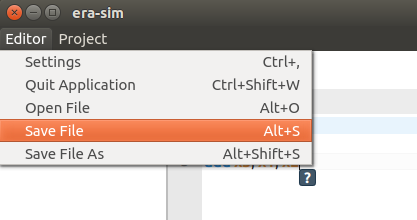
\includegraphics[scale=1.0]{Images/first-steps-7.png}
	\caption{Speichern von Quellcode}
\end{figure}

Ist das geschafft, erstellen wir ein neues Projekt und testen gleich mal das
Laden von Code-Dateien. Dazu gibt es in der Zeile der Projekt-Tabs ein
Plus-Symbol. Dieses öffnet ein neues Tab mit dem schon bekannten
Projekt-Erstellungs-Dialog. Wir vergeben wieder einen Namen, wählen aber diesmal
als Architektur die 64-Bit Version von RISC-V aus.
\begin{figure}[H]
	\centering
	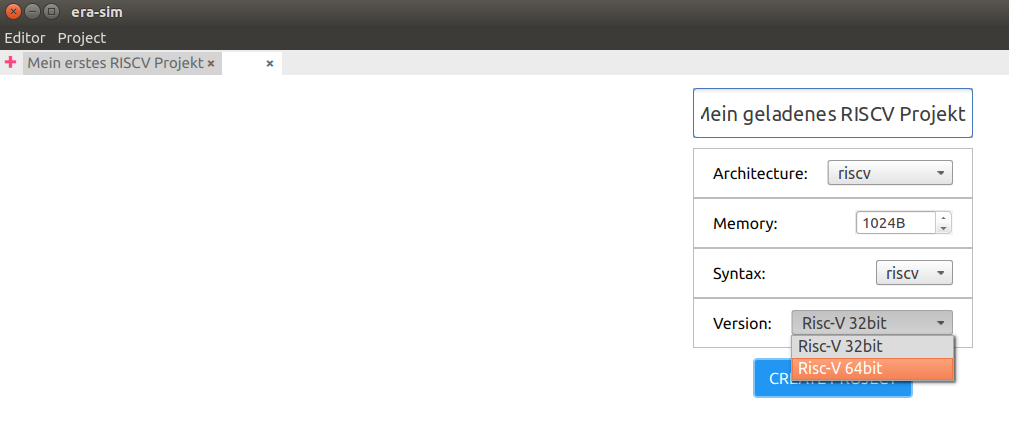
\includegraphics[scale=0.65]{Images/first-steps-8.png}
	\caption{Erstellen eines 64-Bit Projekts}
\end{figure}

Der Mausklick auf ''Create Project'' bringt uns wieder zum Kernstück des
Simulators. Der Unterschied zwischen 32 und 64-Bit scheint subtiler Natur zu
sein, die Komponenten haben sich nicht verändert.  Betrachten wir nochmal die
Registerkomponente. Momentan werden alle Werte der Register als
vorzeichenbehaftete Zahl interpretiert (''S''igned), das sagt jedoch nicht viel
über die Länge des Registers aus. Um diese zu überprüfen, wechseln wir für ein
Register in eine andere Darstellung. Ähnlich wie beim Speicher erlaubt auch hier
ein Klick auf das ''S'' mehrere andere Darstellungsarten. Wir wählen wieder
Hexadezimal.
\begin{figure}[H]
	\centering
	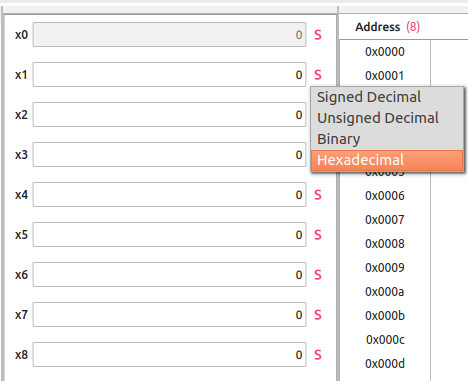
\includegraphics[scale=1.0]{Images/first-steps-9.png}
	\caption{Darstellungsarten der Register}
\end{figure}

Und siehe da, 16 Nullen: $16 \cdot 4$Bit $=64$Bit, passt. Wechseln wir in das
alte 32-Bit Projekt indem wir auf das Tab mit dem Namen ''Mein erstes RISCV
Projekt'' klicken und ändern auch dort die Darstellungsart eines Registers auf
Hexadezimal. Nur 8 Ziffern, also $8 \cdot 4$Bit $=32$Bit.
\begin{figure}[H]
	\centering
	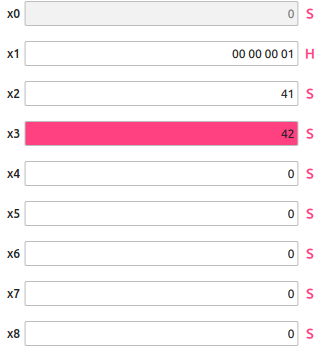
\includegraphics[scale=1.0]{Images/first-steps-10.png}
	\caption{Registerlänge 32-Bit}
\end{figure}

Jetzt wollen wir aber endlich den Code vom alten Projekt laden. Also, zurück zum
64-Bit Projekt und im Dateimenü ''Editor'' den richtigen Eintrag ausgewählt.
\begin{figure}[H]
	\centering
	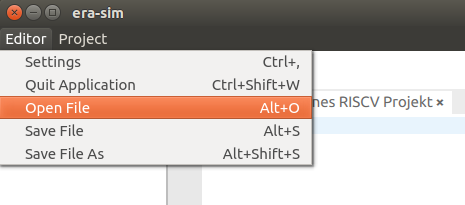
\includegraphics[scale=1.0]{Images/first-steps-11.png}
	\caption{Laden von Quellcode}
\end{figure}

\begin{figure}[H]
	\centering
	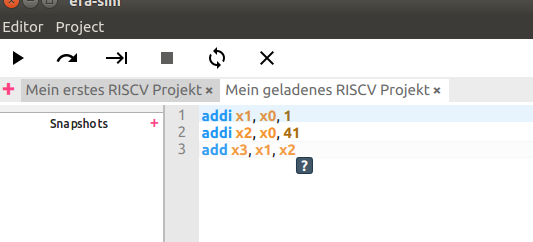
\includegraphics[scale=1.0]{Images/first-steps-12.png}
	\caption{Editor nach dem Laden}
\end{figure}

Der Code ist geladen. Die Register im neuen Projekt sind aber immer noch 0.
Möchte man einen Ausführungszustand speichern (also Registerinhalte bzw.
Speicherinhalt), dann gibt es dafür die Snapshots. Ähnlich wie eine Datei kann
auch ein Snapshot geladen werden. Geladene/Existierende Snapshots werden in der
Snapshot-Komponente auf der linken Seite des Simulators angezeigt und können
dort auch erstellt oder geladen werden. Möchte man von externer Quelle ein
Snapshot laden, geht das auch über das Dateimenü ''Project''.
\begin{figure}[H]
	\centering
	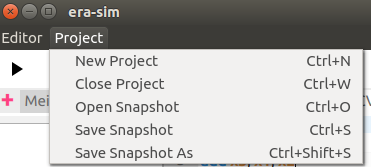
\includegraphics[scale=1.0]{Images/first-steps-13.png}
	\caption{Laden und Speichern von Snapshots}
\end{figure}

Bei Snapshots ist zu beachten, dass diese Architektur- und Modul-gebunden sind.
Ein 32Bit Snapshot kann nicht in ein 64Bit Projekt geladen werden, da hier die
Registergrößen unterschiedlich sind.\\

Damit ist diese kleine Anleitung beendet. Mehr Informationen zu den einzelnen
Komponenten finden sich in den einzelnen Abschnitten. Dort werden alle
Komponenten und auch die RISC-V Architektur genauer beschrieben.
